Inleiding over wat ik vergeleken heb enzo
\subsection{FELICS}
FELICS stands for Fast and Efficient Lossless Image Compression, it is a technique presented by Paul G. Howard and Jeffrey Scott Vitter \cite{felics}.
\begin{figure}[h]
    \centering
    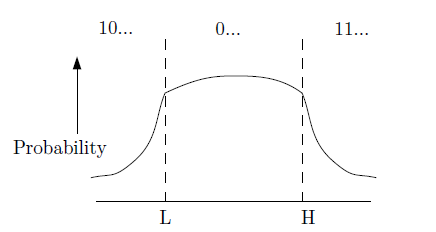
\includegraphics[width=0.25\textwidth]{figs/probability_intensity_P.png}
    \caption{Intensity distribution of new pixel \cite{felics}}
    \label{fig:dist}
\end{figure}
Each pixel is assigned a code depending on where its intensity (gray-scale value) is located relative to the intensities of its closest neigbours. The distribution of an image's intensity distribution is shown in \ref{dist}. L denotes the smaller neigbouring intensity value, H denotes the larger neighbouring intensity value. There are three cases:
\enumerate{
    \item The pixel's intensity P lies in the range [L, H]. One bit (0) is used to indicate the in-range position. Since the values of P are almost uniformly distributed, P is assigned an adjusted binary code that is slightly shorter at the center of the region \cite{handbook}.
    \item The pixel's intensity P is lower than L. Now, one bit (1) is used to indicate the out-of-range position, and one bit (0) is used to indicate the below-range position. 
    \item The pixel's intensity P is higher than H. Now, one bit (1) is used to indicate the out-of-range position, and one bit (1) is used to indicate the above-range position. 
}
The probability of out-of-range values falls off sharply, making it reasonable to use exponential prefix codes like Golomb or Rice codes \cite{felics}.
A formal description of the algorithm can be found in \cite{felics}.